% Copy to docs/ambiguities/lectureNN/main.tex when actual questions arise.
% Replace NN and the title; add real LNN-Qxx entries from the lecture ledger.
% Build from the repository root: make questions LECTURE=NN
% Store evidence crops in the new project's images/ folder.
\documentclass[a4paper,12pt]{article}
\usepackage[margin=19mm]{geometry}
\usepackage{amsmath,amssymb,graphicx,xcolor}
\usepackage{fontspec}
\usepackage{xepersian}
\settextfont{XB Roya}
\setlatintextfont{Latin Modern Roman}
\definecolor{ink}{HTML}{173D75}
\graphicspath{{images/}}
\setlength{\parindent}{0pt}
\setlength{\parskip}{5pt}
\linespread{1.12}
\newcommand{\qtitle}[2]{{\Large\bfseries\color{ink} پرسش \lr{#1}: #2}\par}
\newcommand{\answer}{\par\medskip\textbf{پاسخ یا صورت مورد تأیید و تاریخ:}\par\vspace{18mm}\hrule\medskip}
\begin{document}
{\LARGE\bfseries پرسش‌های ابهام جلسهٔ ۰۷}\par
{\large همریختی‌های مدولی؛ جزوهٔ جبر پیشرفتهٔ دکتر خسروی}\par
شمارهٔ صفحه‌ها یک‌مبنا و مربوط به فایل پی‌دی‌اف است. هر دو پرسش در انتظار پاسخ‌اند؛ اصلاح‌های پیشنهادی هنوز در اسلایدها قطعی نشده‌اند.
\medskip\hrule\medskip

\qtitle{L07-Q01}{دامنه و هم‌دامنهٔ تصویرهای مؤلفه‌ای}
\textbf{وضعیت:} در انتظار پاسخ؛ ثبت در ۲۰۲۶/۱۰/۲۵.\par
\textbf{نشانی منبع:} نسخهٔ \lr{primary}، صفحهٔ ۴، نیمهٔ پایین؛ تعریف \(\pi_1\) و \(\pi_2\) در اثبات قسمت اول.
\begin{LTR}\small\texttt{sources/lectures/07 Hom.pdf}\end{LTR}
\textbf{عبارت منبع:} جزوه برای \(f:N\to M_1\oplus M_2\) می‌گذارد
\[
\psi(f)=(\pi_1\circ f,\pi_2\circ f),
\]
اما در دو سطر بعد، تصویرها را چنین معرفی می‌کند:
\[
\pi_i:\operatorname{Hom}_R(N,M_1)\oplus\operatorname{Hom}_R(N,M_2)
\longrightarrow\operatorname{Hom}_R(N,M_i)\quad(i=1,2).
\]
\begin{center}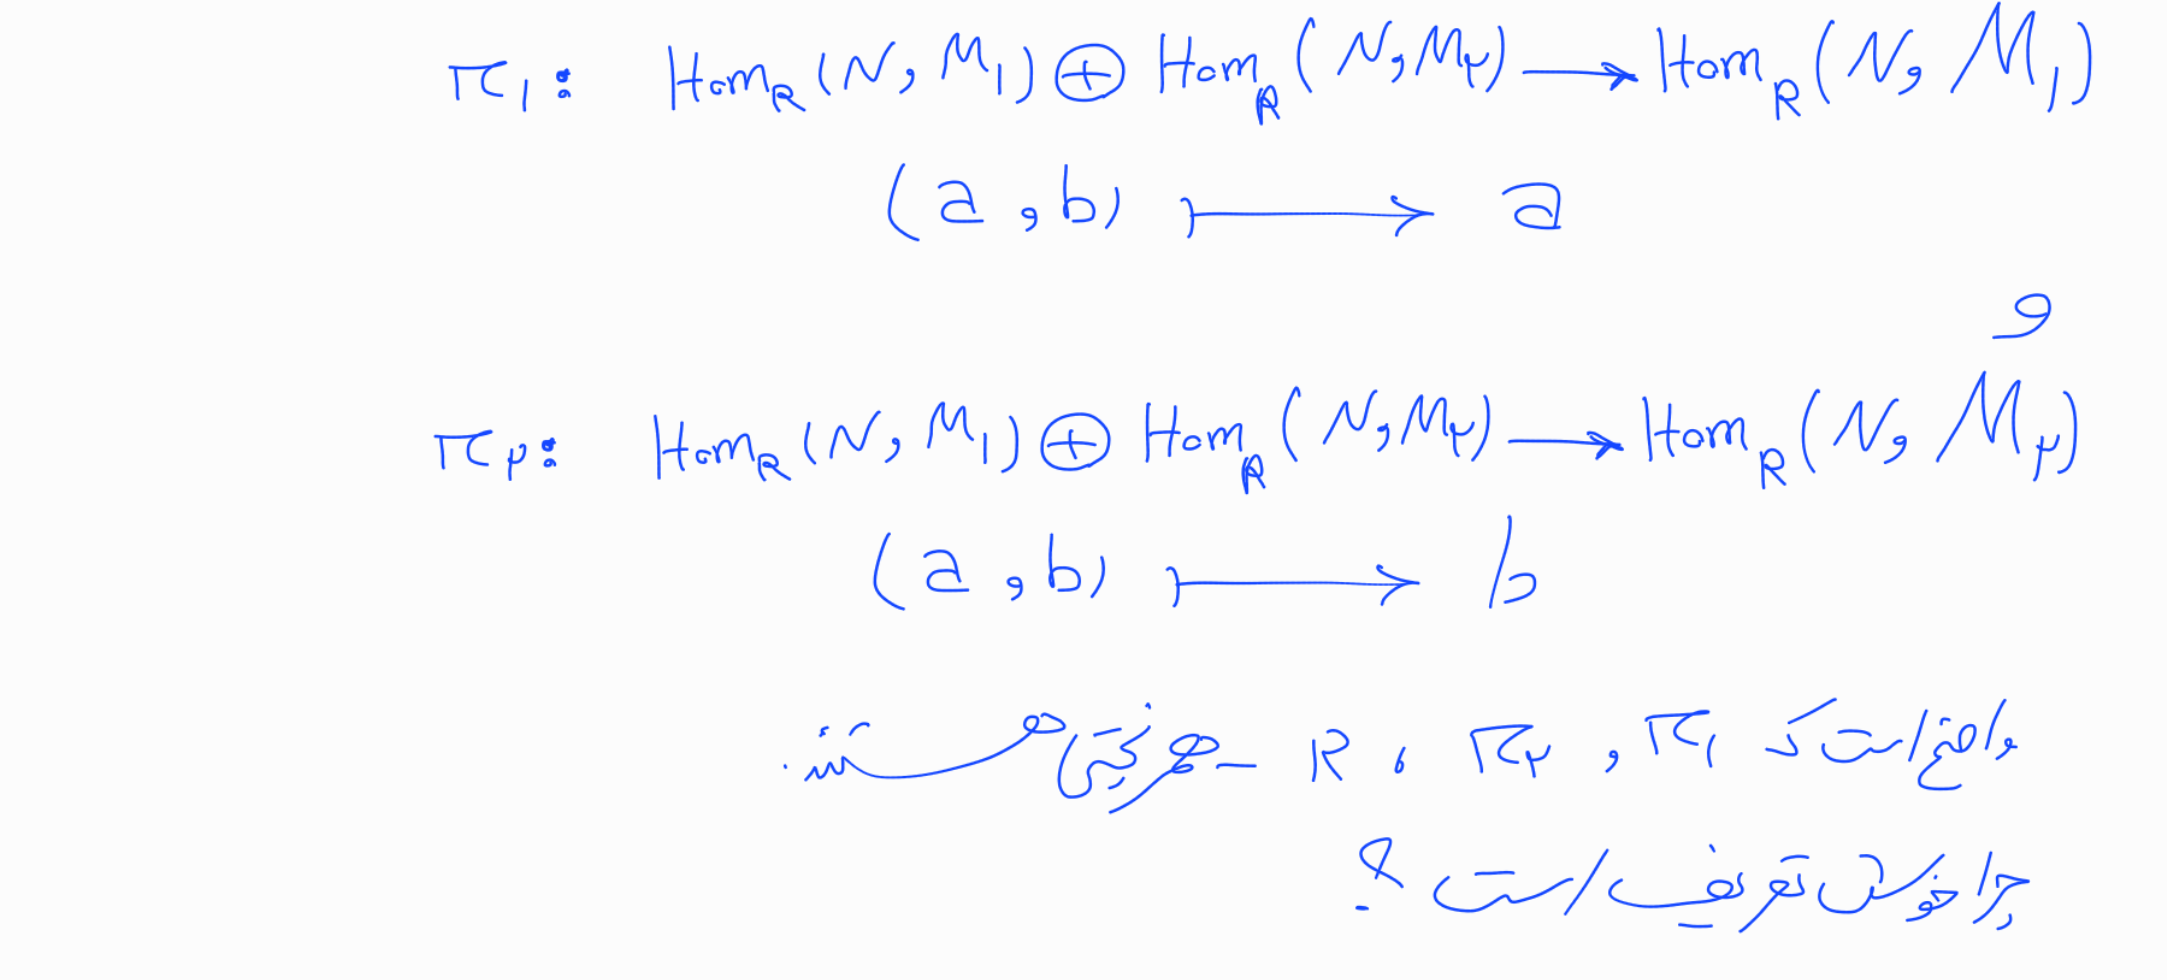
\includegraphics[width=.80\linewidth]{projections.png}\end{center}
\textbf{خوانش‌های ممکن و پیامد:} با تعریف نوشته‌شده، \(\pi_i\circ f\) سازگار نیست؛ زیرا \(f\) در \(M_1\oplus M_2\) مقدار می‌گیرد. ممکن است دامنه و هم‌دامنه اشتباه نوشته شده باشند؛ در غیر این صورت، نگاشت‌ها یا ترکیب دیگری باید مشخص شود.

\textbf{پرسش:} آیا منظور تصویرهای زیر است و آن‌ها را در اسلایدها جایگزین تعریف نوشته‌شده کنم؟
\[
\pi_i:M_1\oplus M_2\to M_i,\qquad
\pi_1(m_1,m_2)=m_1,\quad\pi_2(m_1,m_2)=m_2.
\]
\textbf{پاسخ / تصمیم ثبت‌شده:} هنوز دریافت نشده است.
\answer
\newpage

{\large\bfseries پرسش‌های ابهام جلسهٔ ۰۷؛ ادامه}\par
\medskip\hrule\medskip
\qtitle{L07-Q02}{علامت ناصفربودن مؤلفهٔ دوم}
\textbf{وضعیت:} در انتظار پاسخ؛ ثبت در ۲۰۲۶/۱۰/۲۵.\par
\textbf{نشانی منبع:} نسخهٔ \lr{primary}، صفحهٔ ۵، میانهٔ صفحه؛ بخش یک‌به‌یک بودن، سطر پس از انتخاب عنصری از \(N\) با تصویر ناصفر.
\begin{LTR}\small\texttt{sources/lectures/07 Hom.pdf}\end{LTR}
\textbf{زمینه و عبارت منبع:} ابتدا \(f\in\ker\psi\) فرض شده، پس هر دو نگاشت مؤلفه‌ای صفرند. سپس با فرض \(f\ne0\)، جزوه می‌نویسد
\[
\exists n\in N:\qquad f(n)=(m_1,m_2)\ne(0,0).
\]
در سطر بعد، پس از بازبینی تصویر با وضوح بالاتر، عبارت چنین خوانده می‌شود:
\[
\pi_1\circ f\ne0\quad\text{یا}\quad\pi_2\circ f=0.
\]
\begin{center}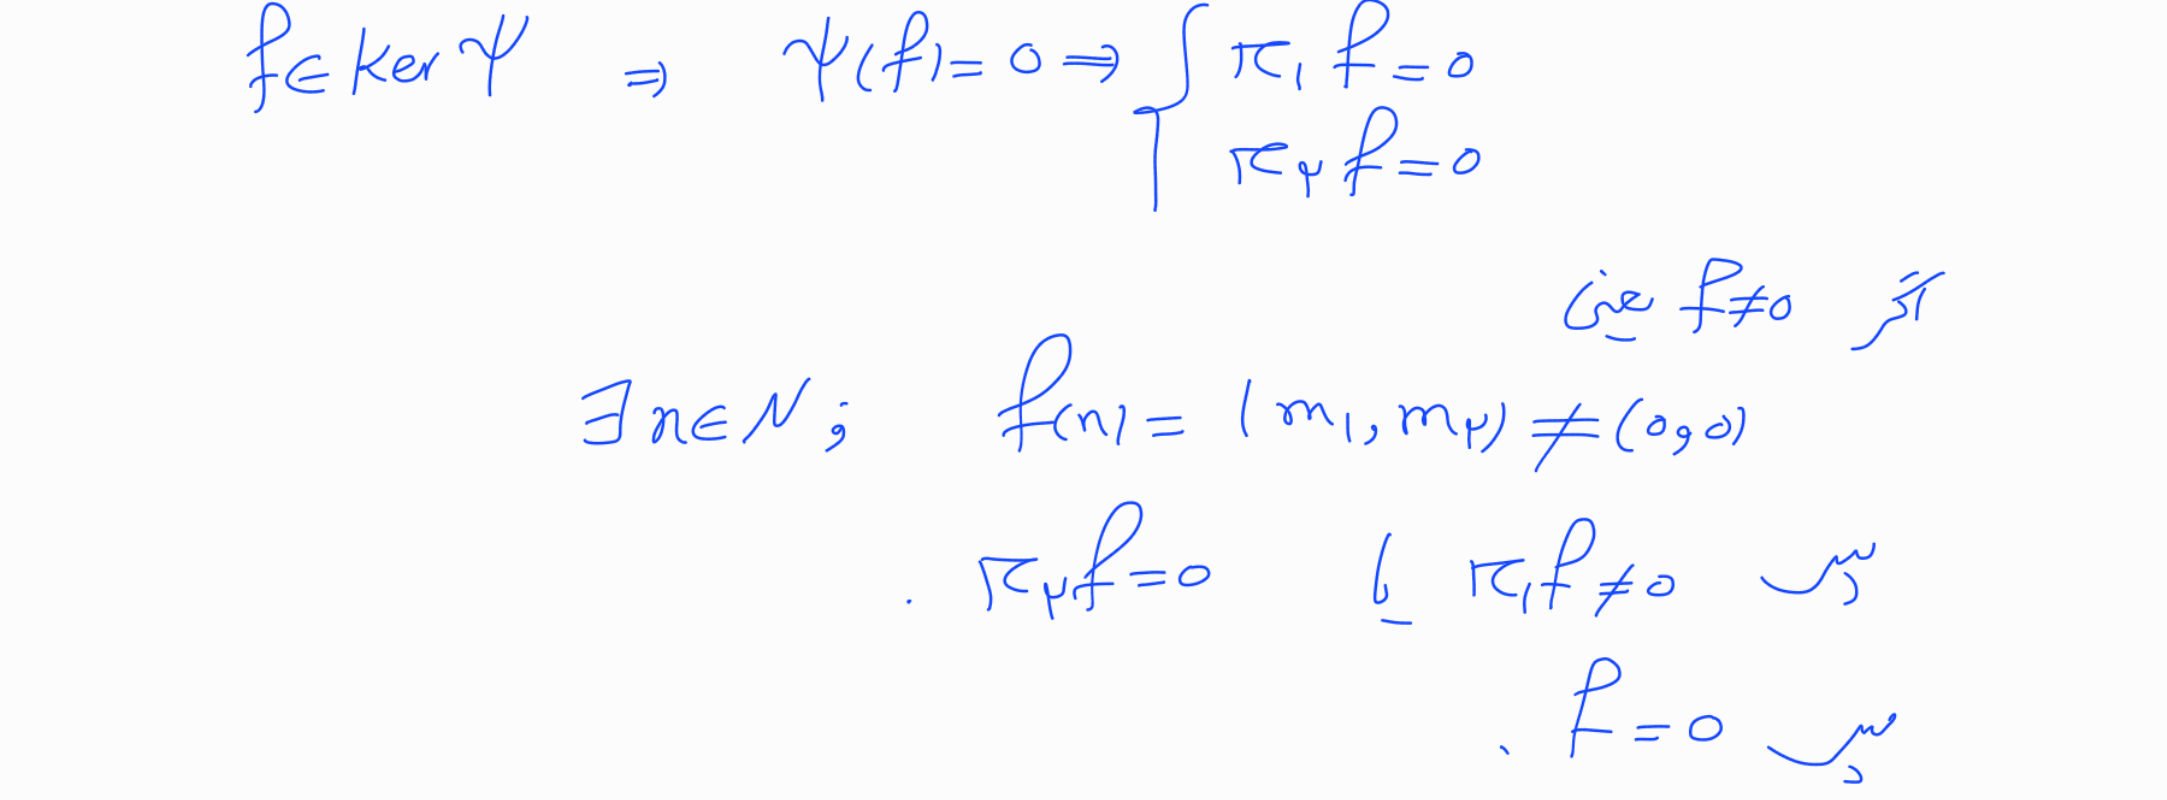
\includegraphics[width=.96\linewidth]{injectivity.png}\end{center}
\textbf{خوانش‌های ممکن:} ممکن است خطِ نابرابریِ رابطهٔ دوم جا افتاده و منظور \(\pi_2\circ f\ne0\) باشد؛ یا استدلال دیگری مد نظر باشد.

\textbf{دلیل پرسش:} عبارتِ ظاهریِ بالا با صفر بودن هر دو نگاشت تناقض ندارد، در حالی که غیرصفر بودنِ دست‌کم یکی از دو نگاشت، گام تناقض را فراهم می‌کند. تعریف خودِ تصویرها نیز موضوع پرسش \lr{L07-Q01} است.

\textbf{پرسش:} آیا رابطهٔ دوم را به نابرابری اصلاح کنم تا این سطر چنین باشد؟
\[
\pi_1\circ f\ne0\quad\text{یا}\quad\pi_2\circ f\ne0.
\]
\textbf{پاسخ / تصمیم ثبت‌شده:} هنوز دریافت نشده است.
\answer
\end{document}
